\subsection{Axis encodings}
\label{sec:axis_encoding}

\textbf{Motivation.} Looking back at the networks generated by \featureset{All} in baseline runs, the learned weigths of most neurons in the feature transformer layer (L1) are related with the movement pattern of the pieces. Let's take the example in Figure \ref{fig:rook_weights}, which depicts the \featureset{Square} part of the features where the role is \symrook\ Rook.

\begin{figure}[h]
\centering
\subfloat[\centering $\white$ White]{{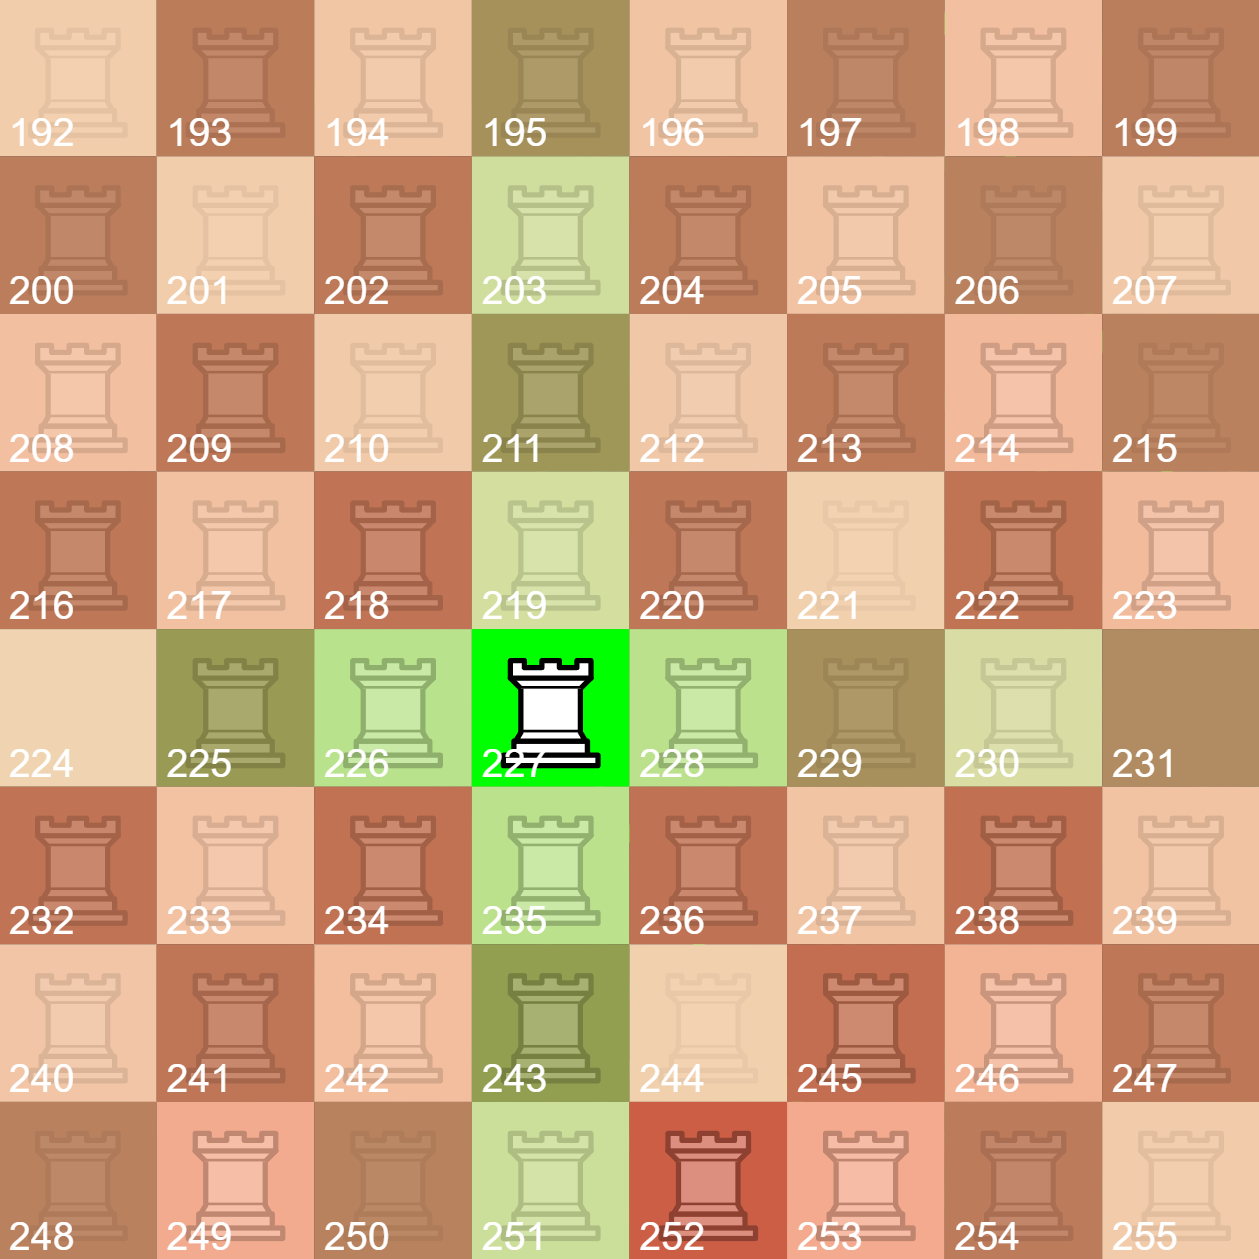
\includegraphics[width=7cm]{../assets/results/piece_weights/white_rook_weights.png} }}%
\qquad
\subfloat[\centering $\black$ Black]{{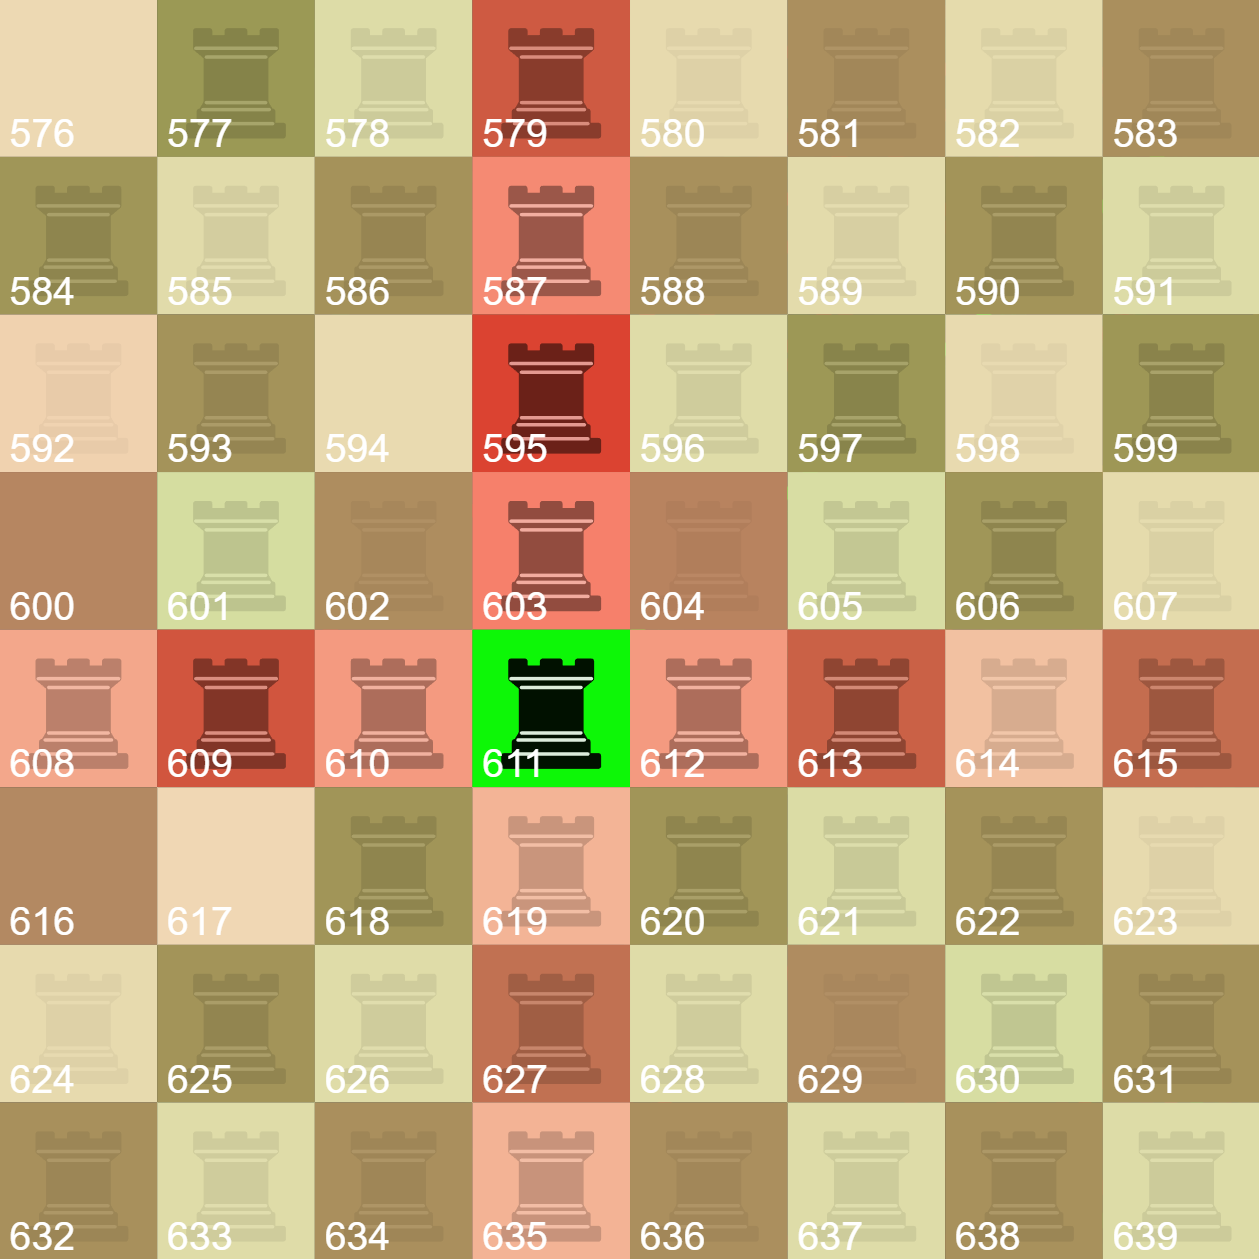
\includegraphics[width=7cm]{../assets/results/piece_weights/black_rook_weights.png} }}%
\caption{Weights of \textbf{a neuron} in the L1 layer, which are connected to features in \featureset{All} where the role is $\rook$ Rook. The intensity represents the weight value, and the color represents the sign (although not relevant).}
\label{fig:rook_weights}
\end{figure}

This particular neuron learned to recognize the presence of a \symrook\ Rook, affected by the pattern of another potential rook in the same file or rank (other pieces may be involved but I am focusing on rooks for the example). Doing so, it had to relate one feature for every potential square where a rook could be for that specific center location, which restrains the network from learning more complex patterns and it is harder to train, because you need more samples to account for all possible combinations.

What if we add a feature which describes \enquote{\textit{there is a $\white$ White $\rook$ Rook in the 4th rank}}? Certainly, this would make the network's job easier, as it would only need to learn the presence of rooks in the corresponding file or rank, instead of every square. This idea can be extrapolated to diagonals, to ease patterns with $\bishop$ Bishops and the $\queen$ Queen.

More examples of this behaviour can be found in Appendix \ref{appendix:axis_samples}, showcasing diagonal patterns and the $\knight$ Knight movements, although they do not move straight through axes. \\

\textbf{Experiment.} I built blocks of features for each natural axis of a chess board, which coincide with the movement pattern of the pieces:

\begin{table}[H]
\centering
\begin{tabular}{cccc}
\depiction{H} & \depiction{V} & \depiction{D1} & \depiction{D2} \\
Horizontal & Vertical & Diagonal 1 & Diagonal 2 \\
(across files) & (across ranks) &  & 
\end{tabular}
\end{table}

% The canonical \featureset{All} feature set encodes each piece's position using the square it is located. Note that this is the same thing as encoding the position for a piece $P$ as $\featureset{File}_{P} \times \featureset{Rank}_{P}$. So the position of each piece is determined using the vertical (across ranks) and horizonal (across files) axes.

In table \ref{tab:axes_blocks} I present the feature blocks. Each block will encode whether there is a piece with the role and color in a specific location along that axis, as explained in the example.

\begin{table}[H]
\caption{Axes feature blocks}
\label{tab:axes_blocks}
\centering

\newcommand{\fullrolecolor}{$\times$ $\featureset{Role}_{P} \times \featureset{Color}_{P}$}

\begin{tabular}{cccccc}
\toprule
\bf Depiction & \bf Block name & \multicolumn{2}{c}{\makecell{\bf Definition\\for every piece $P$ in the board}} & \bf \makecell{Number of\\features} \\
\toprule
\depiction{H} & $\featureset{H}$ & $\featureset{File}_{P}$ & \fullrolecolor & 96 \\
\depiction{V} & $\featureset{V}$ & $\featureset{Rank}_{P}$ & \fullrolecolor & 96 \\
\depiction{D1} & $\featureset{D1}$ & $\featureset{Diag1}_{P}$ & \fullrolecolor & 180 \\
\depiction{D2} & $\featureset{D2}$ & $\featureset{Diag2}_{P}$ & \fullrolecolor & 180 \\
\bottomrule
\end{tabular}

\end{table}


With this blocks, I built different feature sets (listed in table \ref{tab:axis_encoding}): one group of feature sets is just combinations of all the blocks, and another group which is the same as the first but alongside the \featureset{All} feature set (here treated as a block). The second group is the aim of the experiment, it has the classic \featureset{All} feature set but includes the axis blocks to see if the network can benefit from them. The first group, which does not include \featureset{All} is to know how far the network can go only with this blocks alone.

\begin{table}[H]
\caption{Axis encodings feature sets}
\label{tab:axis_encoding}
\centering

\newcommand{\rolecolor}{$\times$ $\featureset{R}_{P} \times \featureset{C}_{P}$}

\begin{tabular}{ccc}
\toprule
\bf Depiction & \bf Feature set & \bf \makecell{Number of\\features} \\
\toprule
\depiction{H} $\oplus$ \depiction{V} & $\featureset{H} \oplus \featureset{V}$ & 192 \\
\midrule
\depiction{D1} $\oplus$ \depiction{D2} & $\featureset{D1} \oplus \featureset{D2}$ & 360 \\
\midrule
\depiction{H} $\oplus$ \depiction{V} $\oplus$ \depiction{D1} $\oplus$ \depiction{D2} & $\featureset{H} \oplus \featureset{V}$ $\oplus$ $\featureset{D1} \oplus \featureset{D2}$ & 552 \\
\midrule
% ------------------------------------
\midrule
\featureset{All} $\oplus$ \depiction{H} $\oplus$ \depiction{V} & $\featureset{All} \oplus \featureset{H} \oplus \featureset{V}$ & 960 \\
\midrule
\featureset{All} $\oplus$ \depiction{D1} $\oplus$ \depiction{D2} & $\featureset{All} \oplus \featureset{D1} \oplus \featureset{D2}$ & 1128 \\
\midrule
\featureset{All} $\oplus$ \depiction{H} $\oplus$ \depiction{V} $\oplus$ \depiction{D1} $\oplus$ \depiction{D2} & \featureset{All} $\oplus$ \featureset{H} $\oplus$ \featureset{V} $\oplus$ \featureset{D1} $\oplus$ \featureset{D2} & 1320 \\
\bottomrule

\end{tabular}
\end{table}

I expect that the feature sets that are sums of single axes ($\depictionSM{H} \oplus \depictionSM{V}, \depictionSM{D1} \oplus \depictionSM{D2}$ and $\depictionSM{H} \oplus \depictionSM{V} \oplus \depictionSM{D1} \oplus \depictionSM{D2}$) will perform worse overall, since to capture the exact position of pieces in the board, the network will have to learn to relate at least two features for every location. This information is already available when \featureset{All} is present.

The feature sets that include \featureset{All} (\featureset{All} $\oplus \hdots$) should perform better than without, providing that the idea explained in the motivation holds.

For each of the proposed feature sets, I will train a network and evaluate its performance relative to each other using a tournament. I expect to see them ranked in the reverse order as presented in the table (more extra axes better). \\

\textbf{Results.} The results in table \ref{tab:axis_results} show that indeed, adding the axes blocks make the network validation loss slightly lower, from 0.00316 in \featureset{All} to 0.00307 including all four blocks. However, this improvement in loss is not significant enough to make the network stronger to compensate the (small) performance hit of having more features. As you can see in the table, including more axes makes the loss decrease slightly yet the rating decreases by a huge factor.

All three feature sets that do not include \featureset{All} unsuprisingly perform much, much worse even having less features. The feature set \featureset{H+V+D1+D2} has a 25\% higher loss than \featureset{All} and $172.5 \pm 4.8$ less rating than \featureset{All}. The other feature sets in this group perform even worse, as it was expected.

I discovered that the accuracy of puzzles is not a good a proxy of an engine's strength, given that there is a 474 rating difference yet 3\% a difference in move accuracy. I believe that the reason lies on the fact that puzzles may be more strategic than positional. I will drop the puzzle accuracy metric in future experiments.

\begin{table}[H]
\caption{Axis encodings results}
\label{tab:axis_results}
\centering

% 1 256-eval_16384_(hv[768]→512)x2→32→1.nn          :     0.0   ----  22665.5   32456    70      96
% 2 256-eval_16384_(hv+h+v[960]→512)x2→32→1.nn      :    -4.6    5.0  22474.0   32456    69     100
% 3 256-eval_16384_(hv+d1+d2[1128]→512)x2→32→1.nn   :   -33.3    5.0  21260.5   32456    66     100
% 4 256-eval_16384_(hv+h+v+d1+d2[1320]→512)x2→32→1.nn   :   -57.7    4.8  20207.5   32458    62     100
% 5 256-eval_16384_(h+v+d1+d2[552]→512)x2→32→1.nn   :  -172.5    4.8  15176.0   32456    47     100
% 6 256-eval_16384_(h+v[192]→512)x2→32→1.nn         :  -368.1    5.7   7527.0   32460    23     100
% 7 256-eval_16384_(d1+d2[360]→512)x2→32→1.nn       :  -474.5    6.4   4289.5   32458    13     ---

% Network: 256-eval_16384_(d1+d2[360]→512)x2→32→1.nn Accuracy: 0.851789055191768
% Network: 256-eval_16384_(h+v+d1+d2[552]→512)x2→32→1.nn Accuracy: 0.8748684518241348
% Network: 256-eval_16384_(h+v[192]→512)x2→32→1.nn Accuracy: 0.8618817235734331
% Network: 256-eval_16384_(hv+d1+d2[1128]→512)x2→32→1.nn Accuracy: 0.8814458606173995
% Network: 256-eval_16384_(hv+h+v+d1+d2[1320]→512)x2→32→1.nn Accuracy: 0.8766955098222639
% Network: 256-eval_16384_(hv[768]→512)x2→32→1.nn Accuracy: 0.8865762394761459
% Network: 256-eval_16384_(hv+h+v[960]→512)x2→32→1.nn Accuracy: 0.8851511342376053

\begin{tabular}{cccccc}
\toprule
\bf Feature set  & \bf \makecell{Number\\of features} & \makecell{\bf Val. loss\\\textit{min}} & \makecell{\bf Rating\\\textit{elo (rel. to \featureset{All})}} & \makecell{\bf Puzzles\\\textit{move acc.}} \\
\toprule
\depiction{H} $\oplus$ \depiction{V} & 192 & 0.00581 & -368.1 $\pm$ 5.7 & 0.8618 \\
\midrule
\depiction{D1} $\oplus$ \depiction{D2} & 360 & 0.00670 & -474.5 $\pm$ 6.4 & 0.8517 \\
\midrule
\makecell{\depiction{H} $\oplus$ \depiction{V} $\oplus$ \\ \depiction{D1} $\oplus$ \depiction{D2}} & 552 & 0.00389 & -172.5 $\pm$ 4.8 & 0.8748 \\
\midrule
% ------------------------------------
\midrule
\featureset{All} (reference) & 768 & 0.00316 & \textbf{0.0} & 0.8865 \\
\midrule
\featureset{All} $\oplus$ \depiction{H} $\oplus$ \depiction{V} & 960 & 0.00308 & -4.6 $\pm$ 5.0 & 0.8851 \\
\midrule
\featureset{All} $\oplus$ \depiction{D1} $\oplus$ \depiction{D2} & 1128 & 0.00309 & -33.3 $\pm$ 5.0 & 0.8814 \\
\midrule
\makecell{\featureset{All} $\oplus$ \depiction{H} $\oplus$ \depiction{V} \\ \hspace{0.75cm} $\oplus$ \depiction{D1} $\oplus$ \depiction{D2}} & 1320 & \textbf{0.00307} & -57.7 $\pm$ 4.8 & 0.8766 \\
\bottomrule

\end{tabular}
\end{table}

The next experiment will focus on adding more specific features, instead of more broad ones.

